\documentclass[11pt, dvipsnames, handout]{beamer}
\newtoggle{full}
\settoggle{full}{true}

\newtoggle{covered}
\settoggle{covered}{false}

\newtoggle{presentable}
\settoggle{presentable}{false}

\newtoggle{dualscreen}
\settoggle{dualscreen}{false}

\usepackage{pgfplots}
%\pgfplotsset{compat = newest}

\usepackage{pgfpages}

\setbeamertemplate{note page}{\pagecolor{yellow!5}\vfill \insertnote \vfill}
\usepackage{collect}
\definecollection{notes}
\newcounter{notestaken}

\usepackage{xpatch}

\usepackage{ulem}

\usepackage[framemethod=tikz]{mdframed}

\usepackage{scalerel}
\usepackage{calc}

%\usepackage{enumitem}
\setlength\fboxsep{.2em}

\usepackage{graphicx} % Allows including images
\usepackage{booktabs} % Allows the use of \toprule, \midrule and \bottomrule in tables

\xpatchcmd{\itemize}
  {\def\makelabel}
  {\setlength{\itemsep}{0.65 em}\def\makelabel}
  {}
  {}


\xpatchcmd{\beamer@enum@}
  {\def\makelabel}
  {\setlength{\itemsep}{0.65 em}\def\makelabel}
  {}
  {}


%\makeatletter
%\renewcommand{\itemize}[1][]{%
%  \beamer@ifempty{#1}{}{\def\beamer@defaultospec{#1}}%
%  \ifnum \@itemdepth >2\relax\@toodeep\else
%    \advance\@itemdepth\@ne
%    \beamer@computepref\@itemdepth% sets \beameritemnestingprefix
%    \usebeamerfont{itemize/enumerate \beameritemnestingprefix body}%
%    \usebeamercolor[fg]{itemize/enumerate \beameritemnestingprefix body}%
%    \usebeamertemplate{itemize/enumerate \beameritemnestingprefix body begin}%
%    \list
%      {\usebeamertemplate{itemize \beameritemnestingprefix item}}
%      {%
%        \setlength\topsep{1em}%NEW
%        \setlength\partopsep{1em}%NEW
%        \setlength\itemsep{1em}%NEW
%        \def\makelabel##1{%
%          {%
%            \hss\llap{{%
%                \usebeamerfont*{itemize \beameritemnestingprefix item}%
%                \usebeamercolor[fg]{itemize \beameritemnestingprefix item}##1}}%
%          }%
%        }%
%      }
%  \fi%
%  \beamer@cramped%
%  \raggedright%
%  \beamer@firstlineitemizeunskip%
%}
%
%
%
%
%
%\makeatother

%\setlist[beamer@enum@]{topsep=1 em}
%\let\origcheckmark\checkmark %screw you dingbat
%\let\checkmark\undefined %screw you dingbat
%\usepackage{dingbat} 
%\let\checkmark\origcheckmark %screw you dingbat






%\usepackage{fontawesome}

\usepackage{mathtools}
\usepackage{etoolbox, calculator}

\usepackage{xcolor}
\usepackage{tikz}
\usetikzlibrary{arrows.meta}
\usetikzlibrary{calc}
\usepackage[nomessages]{fp}
\usepackage{transparent}
\usepackage{accsupp}
%\usepackage{color, xcolor}

%colorblind-friendly palette
%\definecolor{dblue}{RGB}{51,34,136}
\definecolor{lblue}{RGB}{136,204,238}
%\definecolor{green}{RGB}{17,119,51}
\definecolor{tan}{RGB}{221,204,119}
%\definecolor{mauve}{RGB}{204,102,119}

\usepackage{tcolorbox}



\usepackage{xifthen}
\usepackage{nicefrac}
\usepackage{amsmath}
\usepackage{amsthm}
\usepackage{amssymb}
\theoremstyle{definition}
\newtheorem*{define}{Definition}
\newtheorem*{recall}{Recall}


\DeclareMathOperator{\tr}{tr}

\usepackage{multicol}
%\setlength{\columnsep}{1cm}

\usepackage{tablists, amsmath,vwcol, cancel, polynom}
\usetikzlibrary{shapes, patterns, decorations.shapes}
%\usepackage{tikzpeople}
\tikzstyle{vertex}=[shape=circle, minimum size=2mm, inner sep=0, fill]
\tikzstyle{opendot}=[shape=circle, minimum size=2mm, inner sep=0, fill=white, draw]

% common math quick commands
\newcommand{\nicedd}[2]{\nicefrac{\text{d}#1}{\text{d}#2}}
\newcommand{\dd}[2]{\dfrac{\text{d}#1}{\text{d}#2}}
\newcommand{\pd}[2]{\dfrac{\partial #1}{\partial#2}}
\renewcommand{\d}[1]{\text{d}#1}
\newcommand{\ddn}[3]{\dfrac{\text{d}^{#3}#1}{\text{d}#2^{#3}}}
\newcommand{\pdn}[3]{\dfrac{\partial^{#3}#1}{\partial#2^{#3}}}
\newcommand{\p}[0]{^{\prime}}
\newcommand{\pp}[0]{^{\prime\prime}}
\newcommand{\op}[2][\text{L}]{#1 \left[ #2 \right]}

\newcommand{\lap}[1]{\mathcal{L}\left\{#1\right\}}
\newcommand{\lapinv}[1]{\mathcal{L}^{-1}\left\{#1\right\}}
\newcommand{\lapint}[1]{\int_0^\infty e^{-st}#1dt}
\newcommand{\evalat}[2]{\Big|_{#1}^{#2}}

\newcommand{\paren}[1]{ \left( #1 \right)}

\newcommand{\haxis}[4][\normcolor]{\draw[#1, <->] (-#2,0)--(#3,0) node[right]{$#4$}; }


\newcommand{\axis}[4]{\draw[\normcolor, <->] (-#1,0)--(#2,0) 
node[right]{$x$};
\draw[help lines, <->] (0,-#3)--(0,#4) node[above]{$y$};}

\newcommand{\laxis}[6]{\draw[<->] (-#1,0)--(#2,0) 
node[right]{$#5$};
\draw[ <->] (0,-#3)--(0,#4) node[above]{$#6$};}
\newcommand{\xcoord}[2]{
	\draw (#1,.2)--(#1,-.2) node[below]{$#2$};}
\newcommand{\textnode}[3]{
	\draw (#1,#2) node[below]{$#3$};}
	
\newcommand{\nxcoord}[2]{
	\draw (#1,-.2)--(#1,.2) node[above]{$#2$};}
\newcommand{\ycoord}[2]{
	\draw (.2,#1)--(-.2,#1) node[left]{$#2$};}
\newcommand{\nycoord}[2]{
	\draw (-.2,#1)--(.2,#1) node[right]{$#2$};}
\newcommand{\dlim}{\displaystyle\lim}
\newcommand{\dlimx}[1]{\displaystyle\lim_{x \rightarrow #1}}
\newcommand{\stickfig}[2]{
	\draw (#1,#2) arc(-90:270:2mm);
	\draw (#1,#2)--(#1,#2-.5) (#1-.25,#2-.75)--(#1,#2-.5)--(#1+.25,#2-.75) (#1-.2,#2-.2)--(#1+.2,#2-.2);}	

%\newcounter{example}
%\setcounter{example}{1}
%\newcounter{preFrameExample}
%\AtBeginEnvironment{frame}{\setcounter{preFrameExample}{\value{example}}}
%\newcommand{\ex}[1]{
%	 \setcounter{example}{\value{preFrameExample}}
%	 \textcolor{green}{\small\fbox{Example \arabic{example}: #1}}\\[8pt]
%	\stepcounter{example}}
%\newcommand{\exans}[1]{
%	\SUBTRACT{\value{preFrameExample}}{1}{\n}
%	 \textcolor{green}{\small\fbox{Solution \n: #1}}\\[8pt]}
\mode<presentation> {

% The Beamer class comes with a number of default slide themes
% which change the colors and layouts of slides. Below this is a list
% of all the themes, uncomment each in turn to see what they look like.


\usetheme{CambridgeUS}
\usecolortheme[named=black]{structure}


\newcommand{\studentcolor}[0]{ForestGreen}
\newcommand{\normcolor}[0]{NavyBlue}
\newcommand{\alertcolor}{Red}

\setbeamercolor{normal text}{fg=\normcolor}
\setbeamercolor{frametitle}{fg=\normcolor}
\setbeamercolor{section in head/foot}{fg=Black, bg=Gray!20}
\setbeamercolor{subsection in head/foot}{fg=Green!70!Black, bg=Gray!10}
\setbeamercolor{alerted text}{fg=\alertcolor}
\setbeamerfont{alerted text}{series=\bf}
\setbeamertemplate{enumerate items}[default]
\setbeamercolor{enumerate item}{fg=\normcolor}

\setbeamertemplate{footline} % To remove the footer line in all slides uncomment this line
%\setbeamertemplate{footline}[page number] % To replace the footer line in all slides with a simple slide count uncomment this line

\setbeamertemplate{navigation symbols}{} % To remove the navigation symbols from the bottom of all slides uncomment this line
}

\newcommand{\alertbox}[1]{\tcbox[on line, colframe=\alertcolor, colback=White, left=2pt,right=2pt,top=2pt,bottom=2pt]{\usebeamercolor*{normal text}#1}}


\newcommand{\startstu}{\setbeamercolor{normal text}{fg=\studentcolor}\usebeamercolor*{normal text}\setbeamercolor{enumerate item}{fg=\studentcolor}\usebeamercolor*{enumerate item}}
\newcommand{\stopstu}{\setbeamercolor{normal text}{fg=\normcolor}\usebeamercolor*{normal text}\setbeamercolor{enumerate item}{fg=\normcolor}\usebeamercolor*{enumerate item}}

\newcommand{\takenote}[1]{ \begin{collect}{notes}{}{}{}{}  #1  \end{collect}  \addtocounter{notestaken}{1}} %\ifthenelse{\value{notestaken}>0}{\hrulefill\\}{}

\makeatletter
\newcommand{\cover}{\alt{\beamer@makecovered}{\beamer@fakeinvisible}}
\newcommand{\ucover}[1]{\iftoggle{full}{}{\beamer@endcovered}\stopstu#1\startstu\iftoggle{full}{}{\beamer@startcovered}}
\makeatother

\newcommand{\skippause}{ \addtocounter{beamerpauses}{-1}}
\newcommand{\blockpres}{ \skippause \pause }

\newcommand{\studentify}[1]{\startstu #1  \stopstu }
\newcommand{\student}[1]{\iftoggle{full}{ \pause  \studentify{#1} }{\iftoggle{covered}{\studentify{#1}}{\cover{  #1 }}}}
\newcommand{\cstudent}[1]{\student{\begin{center} #1 \end{center}}}
\newcommand{\fullonly}[1]{\iftoggle{full}{ #1}{}}
\newcommand{\presentonly}[1]{\iftoggle{presentable}{ #1}{}}

\usepackage{xparse}
\usepackage{xifthen}

% shortcuts for commonly-used presentation elements
%\NewDocumentCommand{\slide}{o m}
% {\IfValueTF{#1}{\begin{frame}[t]{#1}}{\begin{frame}[t]} #2 \end{frame}}

\newtoggle{iscovered}

\newcommand{\slide}[2][]{%
%\setcounter{notestaken}{0}
\takenote{#2} 
%\ifthenelse{\equal{#1}{}}{\begin{frame}[t]}{\begin{frame}[t]{#1}} #2 \ifthenelse{\value{notestaken}>0}{ \note{\includecollection{notes}}}{} \end{frame}%
\ifthenelse{\equal{#1}{}}{\begin{frame}[t]}{\begin{frame}[t]{#1}} #2 \iftoggle{covered}{\settoggle{iscovered}{true}}{\settoggle{iscovered}{false}}  \note{ \iftoggle{iscovered}{}{\settoggle{covered}{true}} #2 \iftoggle{iscovered}{}{\settoggle{covered}{false}} } \end{frame}%
%\setcounter{notestaken}{0}
}
\newcommand{\defn}[2][]{%
 \setcounter{listcounter}{0}%
\ifthenelse{\equal{#1}{}}{\begin{block}{Definition}}{\begin{block}{#1 :}}%
 #2 \vspace{0.25em} \ifthenelse{\value{listcounter}>0}{\skippause}{} \pause \end{block}%
}



\newcommand{\arr}[2]{\begin{array}{#1}#2\end{array}}
\newcommand{\mat}[2]{\left[\arr{#1}{#2}\right]}
\newcommand{\carray}[1]{\arr{c}{#1}}
\newcommand{\larray}[1]{\arr{l}{#1}}
\newcommand{\rarray}[1]{\arr{r}{#1}}
\newcommand{\colvec}[1]{\mat{c}{#1}}

\newcommand{\itmz}[1]{\addtocounter{listcounter}{1} \begin{itemize}#1 \end{itemize} }
\newcommand{\subitem}[1]{\addtocounter{listcounter}{1} \begin{itemize} \item #1 \end{itemize}}
%
\newcommand{\enum}[1]{\addtocounter{listcounter}{1} \begin{enumerate} #1  \end{enumerate}  }


\newcommand{\algnlbl}[1]{\begin{align}#1  \end{align}} 
\newcommand{\algn}[1]{\begin{align*}#1  \end{align*}} 
\newcommand{\lgn}[1]{ \action<+->{#1} }
\newcommand{\slgn}[1]{\iftoggle{full}{\action<+->{ \startstu #1 \stopstu}}{ \cover{ #1 } } \takenote{$#1$}}

\newcommand{\chckmrk}{\alert{\checkmark}}

\usepackage{pifont}
\newcommand{\xmark}{\alert{\text{\large \ding{55}}}}

\newcommand{\return}[0]{\raisebox{.5ex}{\rotatebox[origin=c]{180}{$\Lsh$}}}
\usepackage{pbox}
%\newcommand{\ex}[1]{\rotatebox[origin=c]{10}{\uline{ex}}:$\;$\pbox[t][][b]{0.9\linewidth}{#1}}
\newcommand{\ex}[1]{\uline{ex}:$\;$\pbox[t][][t]{0.9\linewidth}{#1}}
\newcommand{\eg}[1]{e.g.,$\;$\pbox[t][][t]{0.9\linewidth}{#1}}
\newcommand{\tikzplot}[8][]{%
\begin{tikzpicture}

\begin{scope}[]%
\clip(-#2,-#4) rectangle (#3,#5);%
#8%
\end{scope}%
\laxis{#2}{#3}{#4}{#5}{#6}{#7}%
#1
\end{tikzpicture}%
}


\newcommand{\cancelslide}[1]{%
\begingroup%
\setbeamertemplate{background canvas}{%
\begin{tikzpicture}[remember picture,overlay]%
\draw[line width=2pt,red!60!black] %
  (current page.north west) -- (current page.south east);%
\draw[line width=2pt,red!60!black] %
  (current page.south west) -- (current page.north east);%
\end{tikzpicture}}%
#1%
\endgroup%
}
\renewcommand{\CancelColor}{\color{red}}
\newcommand{\twocols}[3][0.5]{\begin{columns}\begin{column}{#1\textwidth}#2\end{column}\hspace{1em}\vrule{}\hspace{1em}\begin{column}{#1\textwidth}#3\end{column}\end{columns}}

\newcommand{\twomini}[5][1]{\calculatespace \begin{minipage}[t]{\columnwidth}\begin{minipage}[][#1\contentheight][t]{#2\columnwidth}#4\end{minipage}\hfill\begin{minipage}[][#1\contentheight][t]{#3\columnwidth}#5\end{minipage}\end{minipage}}

\newcommand{\threemini}[7][1]{\calculatespace \begin{minipage}[t]{\columnwidth}\begin{minipage}[][#1\contentheight][t]{#2\columnwidth}#5\end{minipage}\hfill\begin{minipage}[][#1\contentheight][t]{#4\columnwidth}#6\end{minipage}\hfill\begin{minipage}[][#1\contentheight][t]{#3\columnwidth}#7\end{minipage}\end{minipage}}


\newcounter{listcounter}
\setcounter{listcounter}{0}



\newif\ifsidebartheme
\sidebarthemetrue

\newdimen\contentheight
\newdimen\contentwidth
\newdimen\contentleft
\newdimen\contentbottom
\makeatletter
\newcommand*{\calculatespace}{%
\contentheight=\paperheight%
\ifx\beamer@frametitle\@empty%
    \setbox\@tempboxa=\box\voidb@x%
  \else%
    \setbox\@tempboxa=\vbox{%
      \vbox{}%
      {\parskip0pt\usebeamertemplate***{frametitle}}%
    }%
    \ifsidebartheme%
      \advance\contentheight by-1em%
    \fi%
  \fi%
\advance\contentheight by-\ht\@tempboxa%
\advance\contentheight by-\dp\@tempboxa%
\advance\contentheight by-\beamer@frametopskip%
\ifbeamer@plainframe%
\contentbottom=0pt%
\else%
\advance\contentheight by-\headheight%
\advance\contentheight by\headdp%
\advance\contentheight by-\footheight%
\advance\contentheight by4pt%
\contentbottom=\footheight%
\advance\contentbottom by-4pt%
\fi%
\contentwidth=\paperwidth%
\ifbeamer@plainframe%
\contentleft=0pt%
\else%
\advance\contentwidth by-\beamer@rightsidebar%
\advance\contentwidth by-\beamer@leftsidebar\relax%
\contentleft=\beamer@leftsidebar%
\fi%
}
\makeatother

\usepackage{circuitikz}
\ctikzset{bipoles/thickness=1.2}

\iftoggle{dualscreen}{\setbeameroption{show notes on second screen=right}}{}
\usetikzlibrary{arrows}

\begin{document}
\section{Lecture 18}
\subsection{Introduction}

\slide[Imagine Hitting a Golf Ball]{\vspace{-1em}

\tikz{\draw (0,0) node{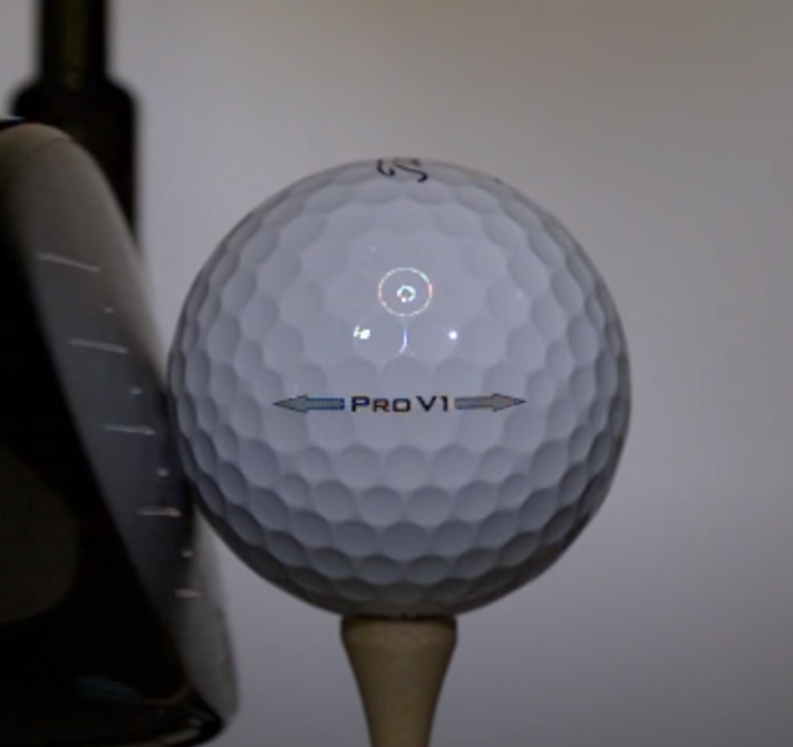
\includegraphics[height=.2\linewidth]{images/golf_ball_1.png}}; \draw[black] (0,-.1) node[fill=white, fill opacity=0.75, text opacity=1, outer sep=0.01, inner sep=1]{\scriptsize$v(0^-)=0$}; }\hfill \tikz{\draw (0,0) node{
\includegraphics[height=.2\linewidth]{images/golf_ball_2.png}}} \hfill \tikz{\draw (0,0) node{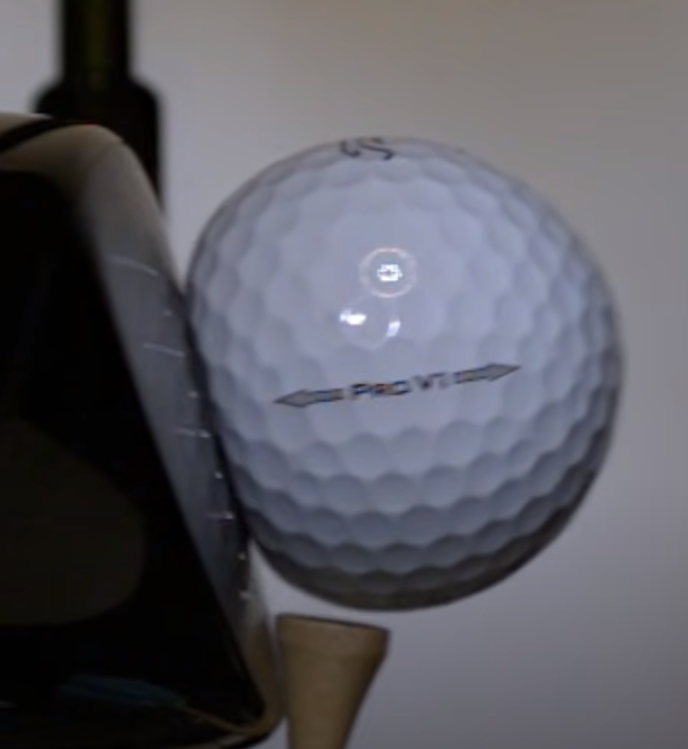
\includegraphics[height=.2\linewidth]{images/golf_ball_3.png}}; } \hfill \tikz{\draw (0,0) node{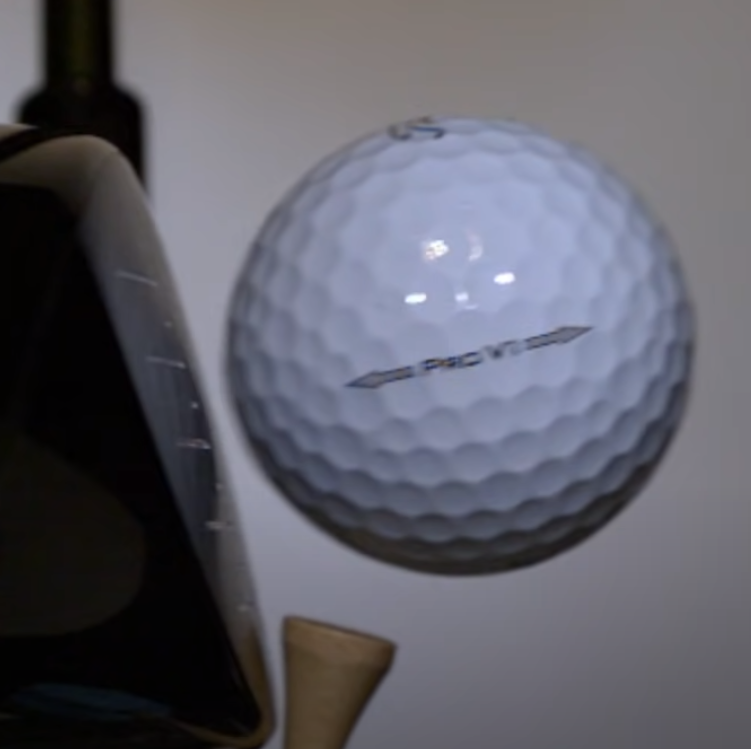
\includegraphics[height=.2\linewidth]{images/golf_ball_4.png}}; \draw[black] (.3,.1) node[fill=white, fill opacity=0.75, text opacity=1, outer sep=0.01, inner sep=1, rotate=30]{\scriptsize$v(0^+)\gg0$}; }

\tiny source:  \url{https://www.youtube.com/watch?v=6TA1s1oNpbk&t=80s}
\normalsize\vspace{-1em}

\twomini[.6]{.6}{.33}{
 \vspace{2em}
The ball is initially at rest, and suddenly a large force is applied to the ball for a very brief period of time.\\~\\
The details of what happens at $t=0$ are too complicated.
}{
\tikzplot[ ]{2}{2}{.3}{3.5}{t}{\text{force}(t)}{

\foreach \xtau in { .08}{
\draw[ultra thick] (-\xtau,0)--(-8,0) ;
\draw[ultra thick] (-\xtau, 0.25/\xtau)--(\xtau,0.25/\xtau) ;
\draw[thick, dashed] (-\xtau,0.25/\xtau)--(-\xtau,0) ;
\draw[thick, dashed] (\xtau,0.25/\xtau)--(\xtau,0) ;
\draw[ultra thick] (\xtau,0)--(6,0) ;

}
}
}\vfill
\student{\centerline{Idea: Approximate the force as an infinitesimally short impulse.}}
}

\subsection{step pulse}
\slide[ Normalized Step Pulse ($\delta_\tau$) ]{
\vspace{-1em}
\newcommand{\hi}{2}
\newcommand{\xtau}{1}
\centerline{
\tikzplot[\xcoord{-\xtau}{-\tau} \xcoord{\xtau}{\tau}  ]{4}{4}{.1}{2.5}{t}{\delta_\tau(t)}{
\draw[ultra thick] (-\xtau,0)--(-5,0) ;
\draw[] (-\xtau,\hi) node[vertex]{};
\draw[ultra thick] (-\xtau, \hi)--(\xtau,\hi) ;
\draw[thick, dashed] (-\xtau,\hi)--(-\xtau,0) ;
\draw[] (-\xtau,0) node[opendot]{};
\draw[thick, dashed] (\xtau,\hi)--(\xtau,0) ;
\draw[] (\xtau,0) node[opendot]{};
\draw[] (\xtau,\hi) node[vertex]{};
\draw[ultra thick] (\xtau,0)--(5,0) ;
\draw[<-] (0.05,\hi-0.1)--(0.3,\hi-0.3) node[right, xshift=-.1cm, yshift=-.1cm]{$\frac{1}{2\tau}$};
}
}
\vfill\student{
\twomini[.3]{.5}{.5}{\uline{Function:}\algn{\delta_\tau &=  \begin{cases} \frac{1}{2\tau} & |t|\leq \tau \\ 0 & |t|>\tau\end{cases} \\ &=\frac{u(t+\tau)-u(t-\tau)}{2\tau}}}{\uline{Integral:} \algn{I(\tau) &=\int_{-\infty}^{\infty} \delta_\tau(t) dt = \int_{-\tau}^{\tau} \frac{dt}{2\tau}\\&=1}}
}}

\slide[Taking the limit $\tau\to0$]{
\newcommand{\hi}{2}
\newcommand{\xtau}{1}
\centerline{
\tikzplot[ ]{8}{4}{.1}{7}{t}{\delta_\tau(t)}{
\student{
\draw[]  (-7,2.75) node{\uline{Integral:}};
\draw[]  (-5,2) node{$\lim_{\tau\to0}I(\tau)=1$};
\draw[]  (-7,6.75) node{\uline{Function:}};
\draw[]  (-5,6) node{$\lim_{\tau\to0}\delta_\tau(t)=\begin{cases} \lim_{\tau \to 0}\frac{1}{2\tau} & t=0 \\ 0 & t\neq0\end{cases} $};
\draw[]  (-4,4.5) node{$=\begin{cases} D.N.E. & t=0 \\ 0 & t\neq0\end{cases}$};
}
\foreach \xtau in {1,.5,.25, 0.125, .08}{
\draw[ultra thick] (-\xtau,0)--(-8,0) ;
\draw[ultra thick] (-\xtau, 0.5/\xtau)--(\xtau,0.5/\xtau) ;
\draw[thick, dashed] (-\xtau,0.5/\xtau)--(-\xtau,0) ;
\draw[thick, dashed] (\xtau,0.5/\xtau)--(\xtau,0) ;
\draw[ultra thick] (\xtau,0)--(6,0) ;
\draw[<-] (\xtau+0.1,0.5/\xtau)--(\xtau+0.3,0.5/\xtau) node[right,]{$\tau=\xtau$};
}
}
}
}

\subsection{Dirac Delta}


\slide[Delta Dirac Function: $\delta(t) \approx \lim_{\tau \to 0} \delta_\tau (t) $]{\vspace{-1em}
\textbf{Theorem:} For any function $f(t)$ that is integrable in some neighbourhood around $c$\[\int_{-\infty}^{\infty} \delta(t-c) f(t) dt = f(c)\]
Integrating against $\delta(t-c)$ essentially "selects" the value of the integrand at $t=c$.
\vfill

More generally
\twomini[.25]{.65}{.35}{
\[\int_a^b \delta(t-c)f(t) dt =\student{ \begin{cases} f(c)& a\leq c\leq b  \\ 0&\text{otherwise}\end{cases}}\]
}{


\tikzplot[\xcoord{0.8}{c}\xcoord{-0.5}{a}, \xcoord{1.5}{b} ]{1.8}{2.2}{.7}{2}{t}{}{

\foreach \xtau in { .01}{
\draw[ultra thick] (0.8-\xtau,0)--(-8,0) ;
\draw[ultra thick] (0.8-\xtau, 0.3/\xtau)--(1+\xtau,0.3/\xtau) ;
\draw[] (0.8-\xtau,0.25/\xtau)--(0.8-\xtau,0) ;
\draw[] (0.8+\xtau,0.25/\xtau)--(0.8+\xtau,0) ;
\draw[] (1.55,1.7) node{$\delta(t-c)$};
\draw[ultra thick] (0.8+\xtau,0)--(6,0) ;
\draw[black, ultra thick, domain=-2:2.2] plot (\x,0.9*\x^2-0.45*\x^3) node[right, above, xshift=-1em, yshift=2em]{$f(t)$};

}
}


}
}

\slide[Sketch of ``proof'':]{

\algn{\int_{-\infty}^{\infty}\delta(t-c)f(t) dt &= \int_{-\infty}^{\infty} \left( \lim_{\tau \to 0} \delta_{\tau}(t-c)\right) f(t) dt\\
&=\lim_{\tau \to 0}  \int_{-\infty}^{\infty}  \delta_{\tau}(t-c) f(t) dt\\
&=\lim_{\tau \to 0}  \frac{1}{2\tau}\int_{c-\tau}^{c+\tau}f(t)dt\\&=\lim_{\tau \to 0} \frac{F(c+\tau)-F(c-\tau)}{2\tau} =f(c)
}
}

\slide[Laplace transform of $\delta(t)$]{
Integrating against $\delta(t-c)$ essentially "selects" the value of the integrand at $t=c$\vfill
Assuming $c>0$
\student{
\algn{\ucover{\lap{\delta(t-c)}=} & \lapint{\delta(t-c) }\\
=&\int_{-\infty}^{\infty} e^{-st} \delta(t-c) dt =e^{-sc}}
}
Special case: $c=0$
\student{\algn{\ucover{\lap{\delta(t)}=\lim_{c \to 0^+}  \lap{\delta(t-c)}} =  \lim_{c \to 0^+}  e^{-sc} = 1 }}

}
\subsection{Example}

\slide[Solve: \hfill $y\pp+6y\p+45y=6\delta(t-5)$ \hfill with $\larray{y(0)=0\\y\p(0)=0}$]{\vspace{-2em}\student{
\algn{
 (s^2+6s+45)Y(s)&= 6e^{-5s} \quad \Rightarrow \quad Y(s) = e^{-5s} \cdot\underbrace{\frac{6}{\underbrace{s^2+6s+45}_{(s+3)^2+36}}}_{\lap{e^{-3t}\sin(6t)}} \intertext{by the convolution theorem}
y(t) &= \delta(t-5) \ast \underbrace{ e^{-3t} \sin \left( 6t \right)}_{f(t)}\\
&=\int_0^t  f(t-\tau) \delta(\tau-5)d\tau\\
&=\begin{cases} 0 & t < 5 \\
f(t-5) &t\geq 5\end{cases}\\
&=u(t-5)f(t-5)
}  
}
}
\subsection{Notes on Dirac Delta}
\slide[Delta Dirac ``Function'': $\delta(t) \approx \lim_{\tau \to 0} \delta_\tau (t) $]{
\itmz{ \item \alert{Note:} $\delta(t)$ is not really well-defined in the conventional sense 
\subitem{It is a "generalized" function with the three following properties: \vfill
\enum{\item $\delta(t)=0$ for $t\neq0$ \vfill  - $\delta_\tau(0) $ D.N.E. in the limit $\tau \to 0$,  which is problematic.\vfill
- Rather than its value, this ``function'' is defined via integral properties \vfill\item $\int_{-\infty}^{\infty} \delta(t) dt =1$ 
\item $\int_a^b \delta(t-c)f(t) dt = \begin{cases} f(c)& a\leq c\leq b  \\ 0&\text{otherwise}\end{cases} $ }
}\vfill
\item The delta function acts like an intense pulse of unit strength. 
\subitem{This is also called an \alert{impulse}: \subitem {An action that happens arbitrarily  fast but with finite magnitude.
 \item ex: accelerating a golf ball with a golf club}}\vfill


}

}

\end{document}